\documentclass[11pt,largemargins]{homework}

\newcommand{\hwname}{Andrew Dudley}
\newcommand{\hwemail}{addudley@asu.edu}
\newcommand{\hwtype}{Homework}
\newcommand{\hwnum}{1}
\newcommand{\hwclass}{CSE 575}
\newcommand{\hwlecture}{}
\newcommand{\hwsection}{}

\usepackage{algorithm}
\usepackage{algpseudocode}
\usepackage{verbatim}
\graphicspath{{images/}}
\newcommand{\argmax}{\operatornamewithlimits{argmax}}
% This is just used to generate filler content. You don't need it in an actual
% homework!
\usepackage{lipsum}

\begin{document}
\maketitle
\question
Suppose that in your coin flip experiment, you observed a set of $\alpha_H$ heads and $\alpha_T$ tails. Let $\theta$ denote the probability of observing heads, whose prior distribution follows $Beta(\beta_H, \beta_T)$, where $\beta_H$ and $\beta_T$ are two positive parameters. 
\begin{alphaparts}
    \questionpart
    Prove that the posterior distribution $P(\theta|D)$ follows $Beta(\beta_H + \alpha_H, \beta_T + \alpha_T)$

	The posterior distribution $P(\theta|D)=\frac{P(D|\theta)P(\theta)}{P(D)}.$ We're told that $$P(\theta)=\frac{\theta^{\beta_H-1}{(1-\theta)}^{\beta_T-1}}{B(\beta_H, \beta_T)} \sim Beta(\beta_H, \beta_T),$$ where $B(\beta_H, \beta_T)$ is the beta function.

	Note that $P(D|\theta)$ is the likelihood function, which for a Bernoulli experiment is $$\theta^{\alpha_H}{(1-\theta)}^{\alpha_T}.$$
	Putting these together, we get $$P(\theta|D)=\frac{\theta^{\beta_H+\alpha_H-1}{(1-\theta)}^{\beta_T+\alpha_T-1}}{P(D)B(\beta_H, \beta_T)},$$
	and because both $P(D)$ and $B(\beta_H, \beta_T)$ are normalizing constants (they don't rely on $\theta$), we can rewrite the equation as 
	$$P(\theta|D)=\frac{\theta^{\beta_H+\alpha_H-1}{(1-\theta)}^{\beta_T+\alpha_T-1}}{B(\beta_H+\alpha_H, \beta_T+\alpha_T)},$$
	From here, we can see that $$P(\theta|D)\sim Beta(\beta_H+\alpha_H, \beta_T+\alpha_T).$$ 
	\questionpart
	What is the mean of $P(\theta|D)$?

	For notational convenience, let $a=\beta_H+\alpha_H$ and $b=\beta_T+\alpha_T$. As they say, statistics is the practice of replacing expectations with averages, so the mean of $P(\theta|D)$ is the same as $\mathbb{E}\left[ P(\theta|D)\right].$ And, of course, because this value is a probability, we can bound the integral by $[0, 1].$
	\begin{align*}
		\mathbb{E}\left[ P(\theta|D)\right] &= \int_{0}^1{\theta P(\theta|D)d\theta} \\
											&= \frac{1}{B(a, v)}\int_0^1{\theta^a{(1-\theta)}^{b-1}d\theta}\\
	\intertext{Here, we can see that the integral is, itself, a beta function.}
	&= \frac{B(a+1, b)}{B(a, b)}\\
	&= \frac{\Gamma(a+1)\Gamma(b)\Gamma(a+b)}{\Gamma(a)\Gamma(b)\Gamma(a+b+1)}\\
	&= \frac{a}{a+b}\\
	&= \frac{\beta_H+\alpha_H}{\beta_H+\alpha_H+\beta_T+\alpha_T}
	\end{align*}

	\questionpart
	What is the MAP estimator $\hat{\theta}_{MAP}\text{ of }\theta?$

	\begin{align*}
		\frac{d}{d\theta}\mathcal{L}(\theta)&=\frac{d}{d\theta}ln\left( \theta^{\beta_H+\alpha_H-1}{(1-\theta)}^{\beta_T+\alpha_T-1}\right)\\
		&= (\beta_H+\alpha_H-1)\left[ \frac{d}{d\theta}ln\theta\right]+(\beta_T+\alpha_T-1)\left[ \frac{d}{d\theta}ln(1-\theta)\right]\\
		&= \frac{\beta_H+\alpha_H-1}{\theta}-\frac{\beta_T+\alpha_T-1}{1-\theta}
	\end{align*}
	And to find a critical point (the minimum value), we set the derivate to 0.
	\begin{align*}
		\frac{\beta_H+\alpha_H-1}{\theta}-\frac{\beta_T+\alpha_T-1}{1-\theta}&=0\\
		\hat{\theta}_{MAP}&=\frac{\beta_H+\alpha_H-1}{\beta_H+\alpha_H+\beta_T+\alpha_T-2}
	\end{align*}
\end{alphaparts}
\question For this question, assume that $x_1, \cdots, x_N\in\mathbb{R}$ are i.i.d. from a normal distribution.
\begin{alphaparts}
	\questionpart Let $\hat{\mu}_{MLE}$ denote the MLE of $\mu$. Prove that $\hat{\mu}_{MLE}$ is unbiased.

	% To prove that $\hat{\mu}_{MLE}$ is unbiased, we must show that $\mathbb{E}[$$\hat{\mu}_{MLE}] = \mu$. Because we're told the data is sampled from a normal distribution, we'll start with the equation of a normal distribution.
	% $$ln(N(x|\mu, \sigma^2)) = -\frac{1}{2}ln(2\pi\sigma^2)-\frac{1}{2\sigma^2}{(x-\mu)^2}$$
	% Also, because the data samples are independent, we then find the log-likelihood of that equation w.r.t $\mu$ to determine $\hat{\mu}_{MLE}$.
	We'll first need to determine the equation for $\hat{\mu}_{MLE}$, then we'll need to compare its expectation to the population mean $\mu$.
	Let $D = \{x_1, \cdots,x_n\}$. Then, because the data is assumed independent, the likelihood of $\mu$ with respect to $D$ can be written as
	$$P(D|\mu)=\Pi_{i=1}^np(x_i|\mu)$$
	Furthermore, we know that the samples are from a normal distribution, giving us
	$$p(x|\mu) = \frac{1}{(2\pi\sigma^2)^{\frac{1}{2}}}e^\frac{(x-\mu)^2}{2\sigma^2}$$
	To simplify finding the derivative, take the log of the likelihood function
	$$\mathcal{L}(P(D|\mu))=\sum_{i=1}^{n}ln(p(x_i|\mu)$$
	Now we'll find the MLE of $\mu$ by taking the derivative of the log-likelihood, setting it to 0, and solving for $\mu$
	\begin{align*}
		\frac{d\mathcal{L}}{d\mu}&=\sum_{i=1}^{n}\frac{d}{d\mu}ln(p(x_i|\mu))&=0\\
		&=-\sum_{i=1}^{n}\frac{d}{d\mu}\left( \frac{1}{2}ln(2\pi\sigma^2)+\frac{1}{2\sigma^2}{(x_i-\mu)^2}\right)&=0\\
		&= \sum_{i=1}^{n}(x_i-\hat{u})&=0\\
		\hat{\mu}&=\frac{1}{n}\sum_{i=1}^{n}x_i
	\end{align*}
	Now that we know the equation for $\hat{\mu}$, we'll find its expectation.
	\begin{align*}
		\mathbb{E}[\hat{\mu}] &= \mathbb{E}\left[\frac{1}{n}\sum_{i=1}^{n}x_i\right]\\
		&= \frac{1}{n}\sum_{i=1}^{n}\mathbb{E}[x]\\
		&= \frac{1}{n}\sum_{i=1}^{n}\mu\\
		&= \mu
	\end{align*}
	Therefore, $\hat{\mu}_{MLE}$ is unbiased.
	\questionpart If the true value of $\mu$ is unknown, then the MLE estimate of $\sigma^2$ is
	$$\sigma^2_{MLE}=\frac{1}{n}\sum_{i=1}^{n}{(x_i-\hat{\mu}_{MLE})}^2$$
	Prove that $\sigma^2_{MLE}$ is biased.

	Before we begin, there are a few derivations that we'll want to have on hand when completing this proof. To start, we'll derive the definition of variance $\sigma^2$.
	
	\begin{align*}
		\sigma^2&=\mathbb{E}\left[ {(X-\mu)}^2\right]\\
		&= \mathbb{E}[X^2-2X\mu+\mu^2]\\
		&= \mathbb{E}[X^2]-2\mu\mathbb{E}[X]+\mu^2\\
		&= \mathbb{E}[X^2]-\mu^2\\
		&= \mathbb{E}[X^2]-{(\mathbb{E}[X])}^2
	\end{align*}
	A little bit of algebraic manipulation of these equations gives us 
	\begin{equation}
		\mathbb{E}{[X^2]}=\sigma^2+\mu^2,
	\end{equation}
	Also note that $\sigma^2$ is a function of X. If we pass into it $\hat{\mu}$, we get
	\begin{align}
		\sigma_{\hat{\mu}}^2&=\mathbb{E}[\hat{\mu}^2]-{(\mathbb{E}[\hat{\mu}])}^2 \nonumber\\
		&=\mathbb{E}[\hat{\mu}^2]-{\mu}^2  
	\end{align}
	We can also derive the variance of $\hat{\mu}$ as follows
	\begin{align}
		\sigma_{\hat{\mu}}^2 &= Var(\frac{x_1+\cdots+x_n}{n}) \nonumber\\
		&=\frac{1}{n^2}Var(x_1+\cdots+x_n)\nonumber\\
		&=\frac{1}{n^2}[Var(x_1)+\cdots+Var(x_n)]\nonumber\\
		&=\frac{\sigma^2}{n}
	\end{align}
	Using (2) and (3), we arrive at the equation
	\begin{equation}
		\mathbb{E}\left[ \hat{\mu}^2\right]=\frac{\sigma^2}{n}+\mu^2
	\end{equation}
	With these derivations in our toolbox, we can now begin the proof that $\sigma^2_{MLE}$ is biased. Again, we'll do so by comparing the expectation of this value to the population variance.
	\begin{align}
		\mathbb{E}\left[ \sigma^2_{MLE}\right] &= \mathbb{E}\left[ \frac{1}{n}\sum{(x_i-\hat{\mu})}^2\right] \nonumber\\
		&= \frac{1}{n}\mathbb{E}\left[ \sum\left( x_i^2-2x_i\hat{\mu}+\hat{\mu}^2\right)\right]\nonumber\\
		&= \frac{1}{n}\mathbb{E}\left[ \sum x_i^2 -2\hat{\mu}\sum x_i+n\hat{\mu}^2\right]\nonumber\\
		&= \frac{1}{n}\mathbb{E}\left[ \sum x_i^2 -2n\hat{\mu}^2+n\hat{\mu}^2\right]\nonumber\\
		&= \frac{1}{n}\left( \sum{\mathbb{E}\left[x_i^2\right]}-n\mathbb{E}\left[\hat{\mu}^2\right]\right)\nonumber\\
		&= \frac{1}{n}\left( n{\mathbb{E}\left[X^2\right]}-n\mathbb{E}\left[\hat{\mu}^2\right]\right)\nonumber\\
		&= \mathbb{E}\left[X^2\right]-\mathbb{E}\left[\hat{\mu}^2\right]
	\end{align}
	Do the expectations in (5) look familiar? They should! Indeed, they are the two expectations that we derived earlier. By plugging the expressions from (1) and (4) into (5), we get
	\begin{align*}
		\mathbb{E}\left[ \sigma_{MLE}^2\right] &= \sigma + \mu^2 - \frac{\sigma^2}{n}-\mu^2\\
		&= \sigma^2 - \frac{\sigma^2}{n}\\
		&= \left(\frac{n-1}{n}\right)\sigma^2
	\end{align*}
	$\left(\frac{n-1}{n}\right)\sigma^2 \neq \sigma^2$, therefore $\sigma_{MLE}^2$ is biased.
\end{alphaparts}
\question
\begin{alphaparts}
	\questionpart How many independent parameters would there be for the Naive Bayes classifier trained with the given data? What are they?

	There would be \textbf{thirteen independent parameters}. Note first that RID is a nominal attribute and buys\_computer is the dependent (target) attribute, leaving us with age, income, student, and credit\_rating as the attributes of interest.

	An assumption is made with Naive Bayes that $$P(X_i|X_{1,\ldots,i-1, x_i+1, \ldots, n}Y)=P(X_i|Y)\forall\, i\,\in\{1, \cdots, n\}$$ 
	A Bayes classifier can be represented as
	$$P(Y_c|X_{1..n})=\frac{P(X_{1..n}|Y_c)P(Y_c)}{\sum_YP(X_{1..n}|Y)P(Y)}$$
	Given the conditional independence assumption of Naive Bayes, this can be simplified to
	$$P(Y_c|X_{1..n})=\frac{\Pi_iP(X_i|Y_c)P(Y_c)}{\sum_YP(X_i|Y)P(Y)}$$

	Let $m_i$ represent the number of discrete categories in the variable $x_i$ and $C$ represent the number of discrete classes of the target attribute Y. Then, given $P(X=X_{ij}|Y=y_c)$ where $j\in \{1, \cdots,m_i\}\text{ and }c\in\{1,\cdots,C\}$, each independent variable $x_i$ contributes $m_i-1$ independent parameters for each class $y_c$. Note that, given $m_i-1$ parameters for the class conditional of an attribute, the final parameter of that class conditional is simply the difference between 1 and the sum of those parameters, and is therefore not independent.
	
	Similarly, we must account for the independent parameters contributed by the prior $P(Y)$, which will be $C-1$ parameters.

	Thus, the equation for the total number of independent parameters in a Naive Bayes model will be
	$$C*\sum_{i=1}^n(m_i-1)+C-1$$

	Plugging in the attributes from the data provided, the number of independent parameters is \textbf{thirteen}.

	\questionpart
	{
		\tiny
		\begin{align*}
			P(age="youth"|buys\_computer="no")=3/5, &P(age="middle\_aged"|buys\_computer="no")=0\\
			P(age="youth"|buys\_computer="yes")=2/9, &P(age="middle\_aged"|buys\_computer="yes")=4/9\\
			P(income="low"|buys\_computer="no")=1/5, &P(income="medium"|buys\_computer="no")=2/5\\
			P(income="low"|buys\_computer="yes")=3/9, &P(income="medium"|buys\_computer="yes")=4/9\\
			P(student="no"|buys\_computer="no")=4/5\\
			P(student="no"|buys\_computer="yes")=3/9\\
			P(credit\_rating)="fair"|buys\_computer="no")=2/5\\
			P(credit\_rating)="fair"|buys\_computer="yes")=6/9\\
			P(buys\_computer="yes")=9/14
		\end{align*}
	}
	\questionpart Given a new person with features $x=(youth, medium, yes, fair)$, what is $P(Y=yes|x)$?

	$$\frac{\frac{2}{9}*\frac{4}{9}*\frac{6}{9}*\frac{6}{9}*\frac{9}{14}}{\frac{2}{9}*\frac{4}{9}*\frac{6}{9}*\frac{6}{9}*\frac{9}{14} + \frac{3}{5}*\frac{2}{5}*\frac{1}{5}*\frac{2}{5}*\frac{5}{14}}=0.80451$$

	Therefore, NB would classify this input at $Y=yes$.
\end{alphaparts}
\question Suppose we have two positive examples $x_1=(1, 0)$ and $x_2=(0, -1)$, and two negative samples $x_3=(0,1)$ and $x_4=(-1, 0).$ Apply standard gradient ascent method to train a logistic regression classifier (without any regularization term). Initialize the weight vector with two different value and set $w_0^0=0$. Would the final weight vector ($w^*$) be the same for the two different initial values? What are the values? You may assume the learning rate to be a positive real constant $\eta$.

For notational and implementation convenience, first append a 1 to each sample vector
\def\pfourmatrix{\begin{bmatrix}
	1 & 0 & 1\\
	0 & -1 & 1\\
	0 & 1 & 1\\
	-1 & 0 & 1
\end{bmatrix}}
$$\left.X=\pfourmatrix\right\}\text{\scriptsize m},\quad\mathbf{\theta}=
\begin{bmatrix}
	0\\
	0\\
	0
\end{bmatrix},\quad\mathbf{y}=
\begin{bmatrix}
	1\\
	1\\
	0\\
	0
\end{bmatrix}$$

$$\mathbf{z}=X\mathbf{\theta}=
\begin{bmatrix}
	0\\
	0\\
	0\\
	0
\end{bmatrix},\quad\mathbf{\hat{p}}=sig(\mathbf(z))= \frac{1}{1+e^{-z}}=
\begin{bmatrix}
	0.5\\
	0.5\\
	0.5\\
	0.5
\end{bmatrix}$$
$\textbf{$\hat{p}$}$ represents the model's estimated probabilities of a positive class in vectorized form. When performing prediction, a threshold value of 0.5 is set such that the predicted class is 1 when $p>0.5$ and 0 when $p\leq 0.5$. This threshold effectively draws a discriminant line in the input space. When training, however, The cross-entropy loss is used as a cost function on the estimated probability. When training with batches of data, the total loss is simply the average cost over the training data. This allows us to write the cost function as
$$J(\mathbf{\theta})=-\frac{1}{m}\sum_{i=1}^my^{(i)}log(\hat{p}^{(i)})+(1-y^{(i)})log(1-\hat{p}^{(i)})$$
To minimize the loss, we can calculate the gradient of $J(\mathbf{\theta})$ with respect to $\mathbf{\theta}$ and then update $\mathbf{\theta}$ in the negative direction of that gradient. Iterating over this process ad infinitum will converge to the optimal parameters (ignoring issues of perfect separation, etc).
$$\frac{\delta J(\mathbf{\theta})}{\delta \theta_j}=\frac{\delta J}{\delta \hat{p}}\frac{\delta \hat{p}}{\delta z}\frac{\delta z}{\theta_j}$$
\begin{align*}
	\frac{\delta J}{\delta\hat{p}} &= -\frac{1}{m}\sum_{i=1}^m\left[\frac{y^{(i)}}{\hat{p}^{(i)}}-\frac{1-y^{(i)}}{\hat{1-p}^{(i)}}\right]\\
	&= -\frac{1}{m}\sum_{i=1}^m\left[ \frac{y^{(i)}-\hat{p^{(i)}}}{\hat{p}^{(i)}(1-\hat{p}^{(i)})}\right]
\end{align*}
\begin{align*}
	\frac{\delta\hat{p}}{\delta z}&= sig(z)(1-sig(z))\\
	&= \hat{p}(1-\hat{p})
\end{align*}
$$\frac{\delta J}{\delta\hat{p}}\frac{\delta\hat{p}}{\delta z}=\frac{1}{m}\sum_{i=1}^m\hat{p}^{(i)}-y^{(i)}$$
$$\frac{\delta z}{\delta\theta_j}=x_j$$
$$\frac{\delta J}{\delta \hat{p}}\frac{\delta \hat{p}}{\delta z}\frac{\delta z}{\theta_j}=\frac{1}{m}\sum_{i=1}^m(\hat{p}^{(i)}-y^{(i)})x_j^{(i)}$$  
From this result, it is clear that the only calculation we need to complete prior to updating our weights is the sigmoid function.
It's also worth noting that this result can be written in matrix form, which allows for efficient computation when implementing
$$\frac{\delta J}{\delta \hat{p}}\frac{\delta \hat{p}}{\delta z}\frac{\delta z}{\theta}=\frac{1}{m}X^T(\hat{p}-y)$$
Now that we know the process of logistic regression, what can we say about the parameters? What do they represent?

Unfortunately, interpreting the parameters learned isn't nearly as straight forward as it is in linear regression models, even though what we're ultimately fitting is a discriminant line in the feature space. However, if we consider the threshold value 0.5 and its relation of the the input to the sigmoid function z, we know that when $z > 0,\,sig(z) > 0.5$. Likewise, when $z\leq 0, \, sig(z) \leq 0.5$. From this, it is obvious that the parameters we are learning are for a line in the feature space at form at $z=0$. Scaling the coefficients of z by any scalar value would result in the same line, so the there are infinite values that $\theta$ could converge to, and this will depend on the the values that the vector is initiated with.


In this example, the values will ultimately converge to $\theta_1=-\theta_2$ (s.t. $\theta_1\in\mathcal{R}$), and $b=0$
$$\theta_1x_1+\theta_2x_2+b=0$$

\question{Naive Bayes Classifier and Logistic Regression}
\begin{alphaparts}
	\questionpart
	- How many independent parameters are there in this Gaussian Naive Bayes classifier? What are they?

	Unlike Question 3, the class-conditionals in this problem aren't discrete, they're probability distribution functions. There are infinite possible values of $x_i$, and therefore no notion have having ``$m_i-1$'' independent variables per attribute. Instead, each attribute has a corresponding $\mu$ and $\sigma^2$ parameter for each of the two possible class labels. However, because the target attribute is still discrete (boolean), one of the priors constitutes an independent parameter and the other does not.

	Thus, there are $9$ independent parameters in this problem.

	- Can we translate $w$ in to the parameters of an equivalent Gaussian Naive Bayes classifier without any extra assumption?\\
	{\footnotesize\bf
		Note:  Tom Mitchell's Machine Learning book was referenced for this problem.
		{\itshape 
			Machine Learning, Tom Mitchell, McGraw Hill, 1997.
		}
	}


	To determine a relationship between Gaussian Naive Bayes and logistic regression, it would help to first have them in a similar form. 
	
	The posterior probability of the positive class in Naive Bayes is, by definition

	$$\frac{P(D|Y=1)P(Y=1)}{P(D|Y=1)P(Y=1)+P(D|Y=0)P(Y=0)}$$

	By dividing the numerator and denominator by the numerator, we get
	$$\frac{1}{1+\frac{P(X|Y=0)P(Y=0)}{P(X|Y=1)P(Y=1)}}$$

	Which can be written as
	
	\begin{align*}
		\frac{1}{1+e^{ln\left(\frac{P(X|Y=0)P(Y=0)}{P(X|Y=1)P(Y=1)}\right)}} &= \frac{1}{1+e^{ln\left( \frac{P(Y=0)}{P(Y=1)} \right) + \sum_i ln\left( \frac{P(X_i|Y=0)}{P(X_i|Y=1)} \right)}} \\
	\end{align*}
	
	Notice that $\frac{P(Y=0)}{P(Y=1)}$ is the definition of odds, and can be written as $\frac{p}{1-p}$.

	$$\frac{1}{1+e^{ln\left( \frac{p}{1-p} \right) + \sum_i ln\left( \frac{P(X_i|Y=0)}{P(X_i|Y=1)} \right)}}$$

	Now, let's unpack the summation to reveal the parameters of the NB classifier\ldots

	\begin{align*}
		\sum_iln\frac{P(X_i|Y=0)}{P(X_i|Y=1)} &= \sum_iln \frac{\frac{1}{\sqrt{2\pi\sigma_i^2}}exp \left( \frac{-(X_i-\mu_{i0})^2}{2\sigma_i^2} \right)}{\frac{1}{\sqrt{2\pi\sigma_i^2}}exp \left( \frac{-(X_i-\mu_{i1})^2}{2\sigma_i^2} \right)} \\
		&= \sum_i \left( \frac{\mu_{i0}-\mu_{i1}}{\sigma_i^2}X_i + \frac{\mu_{i1}^2-\mu_{i0}^2}{2\sigma_i^2} \right)
	\end{align*}

	Plugging the summation back into the original equation, we have
	$$\frac{1}{1+e^{ln\left( \frac{p}{1-p} \right) + \sum_i \left( \frac{\mu_{i0}-\mu_{i1}}{\sigma_i^2}X_i + \frac{\mu_{i1}^2-\mu_{i0}^2}{2\sigma_i^2} \right)  }}$$

From here, we can see in the exponent that we have a linear combination of the $X_i$ vectors in terms of the parameters of Naive Bayes, along with a constant value

 $$w_0 = \ln\left( \frac{p}{1-p} \right)+ \sum_i \frac{\mu_{i1}^2-\mu_{i0}^2}{2\sigma_i^2}$$ 

 $$w_i= \frac{\mu_{i0}-\mu_{i1}}{\sigma_i^2} $$

	\questionpart
\textbf{Implementation of Naive Bayes and Logistic Regression.} Compare the two approaches on the bank note authentication dataset. Implement a Gaussian Naive Bayes classifier and a logistic regression classifier. Please write you code from scratch. For the NB classifier, assume the $P(x_i|y)\sim\mathcal{N}(\mu_{i, k}, \sigma_{i, k})$ where $x_i$ is a feature in the bank note data and $y$ is the class label. Use three-fold cross-validation to splite the data and train/test your models.
\begin{arabicparts}
	\questionpart
	For each algorithm: briefly describe how you implement it by giving the pseudocode. The pseudocode must include equations for estimating the model parameters and for classifying a new sample.
	
	\begin{algorithm}
		\caption{Logistic regression}
		\begin{algorithmic}
			\Procedure{train}{$X, y, \theta$}\Comment Train the model
				\For{$i \gets 1, 1000$}
				\State $\mathbf{z}\gets X\mathbf{\theta}$
				\State $\mathbf{p} \gets sigmoid(\mathbf{z})$
				\State $\Delta\mathbf{\theta}=mean(diag(\mathbf{p}-\mathbf{y})X)$
				\State $\mathbf{\theta}=\mathbf{\theta} - \Delta\mathbf{\theta}$
				\EndFor
				\State \textbf{return $\theta$}
			\EndProcedure
			\item[]
			\Procedure{predict}{$x, \theta$}
				\State $z\gets x\cdot\mathbf{\theta}$
				\State $p \gets sigmoid(z)$
				\If{$p > 0.5$}
				\State $\mathbf{return \quad 1}$
				\Else
				\State $\mathbf{return \quad 0}$
				\EndIf
			\EndProcedure
		\end{algorithmic}
	\end{algorithm}
	\begin{algorithm}
		\caption{Naive Bayes}
		\begin{algorithmic}
			\Procedure{train}{$X, y$}
				\State $\mathbf{\mu_{j, c}} \gets mean(\{x_{i, j} |y_i = c\})\quad \forall c \in unique(y)$
				\State $\mathbf{\sigma^2_{j, c}} \gets variance(\{x_{i, j} |y_i = c\}) \quad \forall c \in unique(y)$
				\State $\mathbf{p} \gets length(\{y_{i}|y_{i}=c\})/length(\mathbf{y}) \quad \forall c \in unique(y)$
				\State \textbf{return $\mu, \sigma, p$}
			\EndProcedure
			\item[]
				\Procedure{predict}{$x, \mathbf{\mu}, \mathbf{\sigma}, \mathbf{p}$}
			\State $\mathcal{L}_c = \Pi_j \, \mu_{j,c}$	
			\State $\mathbf {\textbf{return} \argmax_c(\mathcal{L}_c*\mathbf{p}_c)}$
			\EndProcedure
		\end{algorithmic}
	\end{algorithm}
	\questionpart
	Plot a learning curve: The accuracy vs the size of the training set. Plot 6 points for the curve, using $[0.01, 0.01, 0.05, 0.1, 0.625, 1]$ random fractions of your training set, and testing on the full test set each time. Average your results over 5 runs using each random fraction of the training set. Plot both the Naive Bayes and the logistic regression learning cureves on the same figure. 

	\begin{center}
		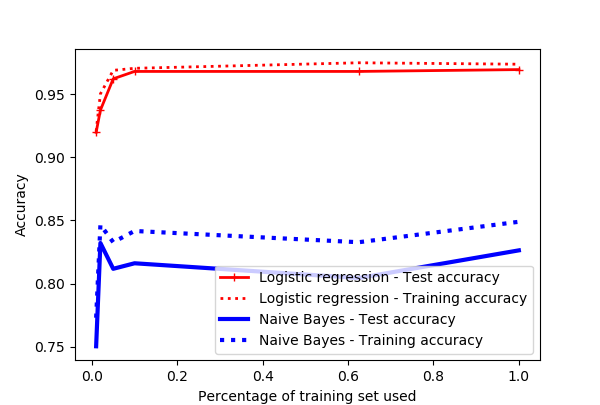
\includegraphics[scale=0.7]{Figure_1.png}
	\end{center}
	\questionpart
	Show the power of the generative model: Use your trained Naive Bayes classifier to generate 500 examples from class $y=1$. Report the mean and variance of the generated examples and the corresponding training data (for each fold, over 1 run). Compare the results with the parameters learned from the training set.

	My implementation uses the unbiased variance estimator (sample variance). The learned parameters and the parameters of the generated data are very similar, which is to be expected, as the generated data is generated using the learned parameters.
	\verbatiminput{results.txt}
\end{arabicparts}
\end{alphaparts}

\end{document}
